\subsection{Generator Training}
To evaluate the performance of the StyleGAN2-Ada generator, multiple evaluation metrics have been computed for different snapshots saved during training. Training curves for the StyleGAN2-Ada model can be found in the appendix in figure \ref{fig:sg2ada_evaluation_metrics}. FID and KID are at the lowest at step 1200, meaning after 1200k images have been shown to the discriminator. Interestingly, IS shows the highest value at step 1800. Since the value at step 1200 is also fairly high and IS is less meaningful for the task at hand as described in section \ref{sec:gan_evaluation}, this discrepancy is ignored. Looking at the Precision and Recall curves, Precision, i.e. the fraction of realistic-looking images peaks early at step 600 while Recall, i.e. the diversity of generated images peaks at step 1200. Since there is an inherent trade-off between the two, I choose higher diversity while accepting a slightly lower fidelity in the generations. Consequently, step 1200 is chosen as the model to be used in all downstream applications.
\begin{figure}[ht!]
    \centering
    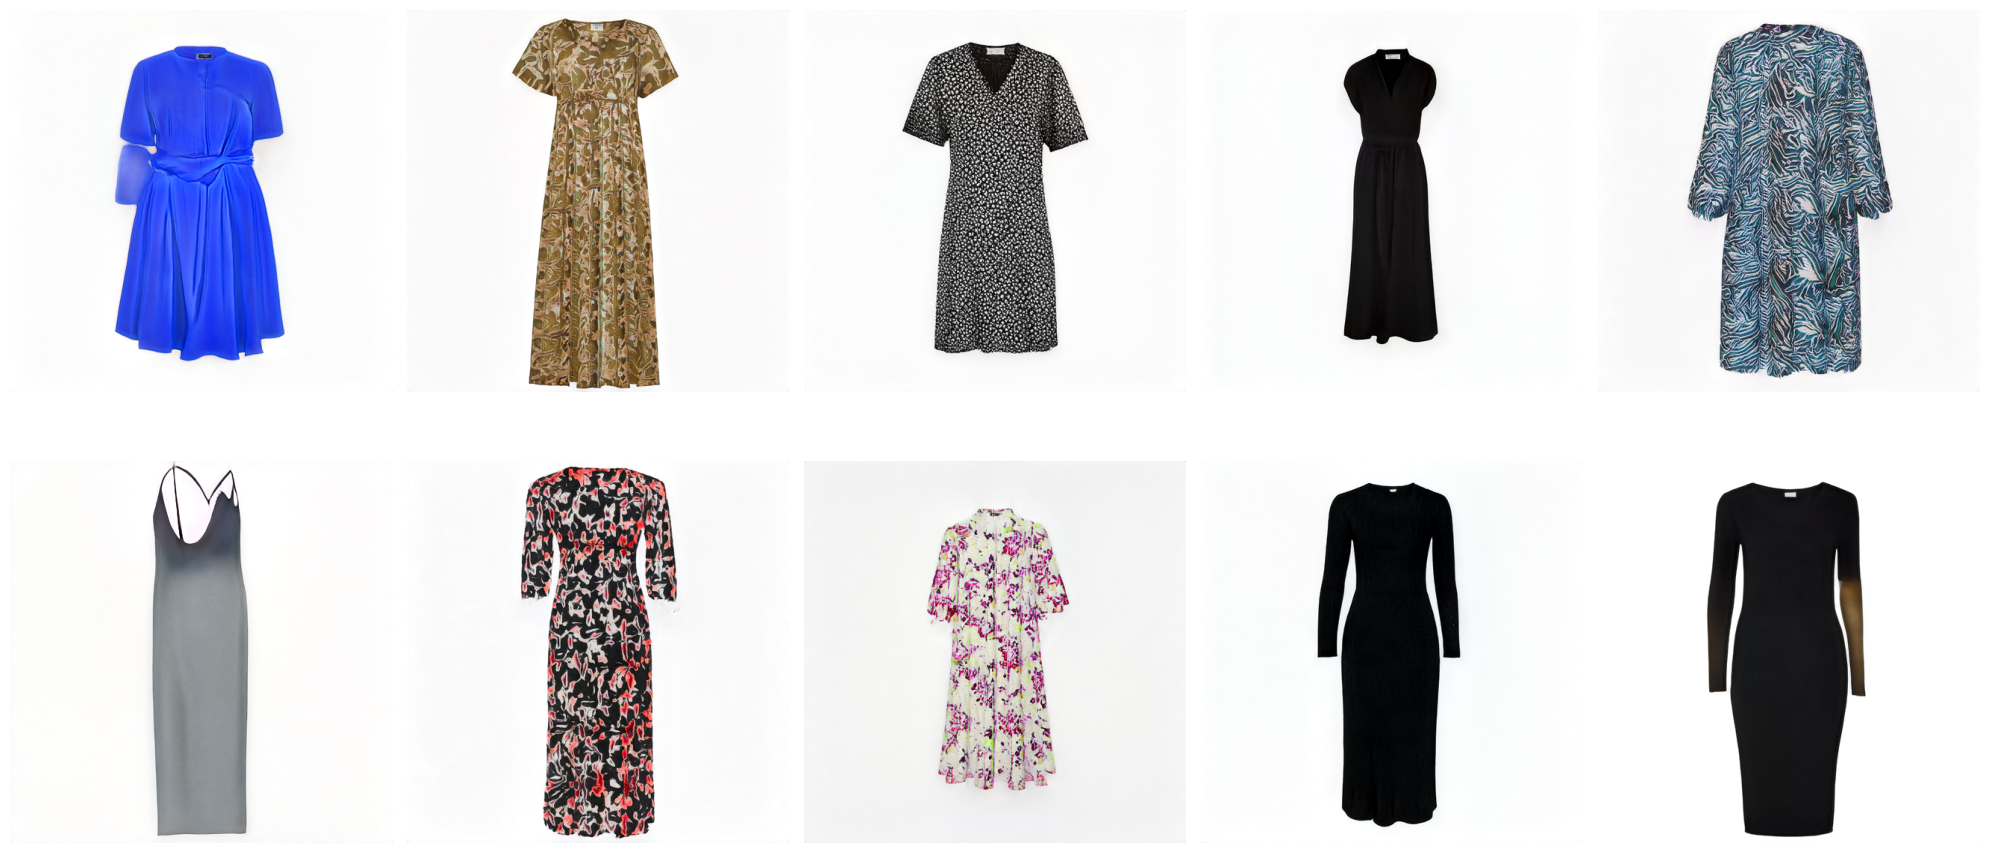
\includegraphics[width=1\linewidth]{Thesis/Results/assets/generated_samples.png}
    \caption[Generated Dresses from StyleGAN2-Ada Model]{Generated Dresses from StyleGAN2-Ada Model \textit{The random generation showcases the diversity of dresses that the generator is capable of generating. At the same time, some generations may exhibit artifacts like the two different sleeve lengths in the upper left image.}}
    \label{fig:generated_samples}
\end{figure}

To validate the training results, both a quantitative evaluation against comparable models in literature as well as a qualitative evaluation are conducted. With a final FID score of 8.09, the generator performance lies exactly in the range of 7.5-10.0 which has been established in the original StyleGAN2-Ada paper for datasets with comparable sizes \citep[p.8]{stylegan2}. Other applications of StyleGAN2-Ada have similar FID scores (e.g. 8.7 in \cite{fu2022stylegan}) or much higher scores (e.g. 13.68 in \cite{hermosilla2021thermal} and 26.02 in \cite{kim2022effective}). A similar application that aims at clothing generation could achieve an FID of 4.53 using a conditional StyleGAN2-Ada model and training on a much larger dataset of 62k images for ten days. Given those benchmark results, the FID achieved for my StyleGAN2-Ada model is well in the range of applications with similar dataset sizes and computational resources used. For a qualitative evaluation of the images generated by the final model, please refer to figure \ref{fig:generated_samples}.


